%! Author = matteomagnini
%! Date = 05/03/25

%----------------------------------------------------------------------------------------
\chapter{Neuro-symbolic AI}
\label{ch:nesy-ai}
\minitoc
%----------------------------------------------------------------------------------------

The origins of \gls{NeSy} \gls{AI} can be traced back to the 1950s and 1960s, during the early days of \gls{AI} research~\cite{Youheng_2023}.
%
At that time, the focus was on developing systems based on symbolic reasoning and rule-based problem-solving.
%
However, by the 1980s, the limitations of purely symbolic approaches became evident.
%
For instance, symbolic \gls{AI} struggled with tasks such as \gls{NLP} and computer vision, where the complexity of real-world data posed significant challenges.
%
To address these shortcomings, researchers began incorporating principles inspired by neuroscience into \gls{AI} systems.
%
This shift marked the beginning of efforts to integrate sub-symbolic methods, such as neural networks, into the field.

In the early 21st century, the idea of combining symbolic reasoning with neural networks gained traction.
%
This led to the emergence of \gls{NeSy} \gls{AI}, a hybrid approach that leverages the strengths of both symbolic and sub-symbolic paradigms.


\Gls{NeSy} \gls{AI} has since been applied to a wide range of domains, including healthcare, robotics, and \gls{NLP}.
%
It represents one of the most promising directions in \gls{AI} research, aiming to create systems capable of both learning from data and reasoning logically, much like humans.
%
The ``neuro'' component of \gls{NeSy} \gls{AI} is inspired by the human brain's ability to process information and learn from experience.
%
This is achieved through the use of neural networks, which enable the system to adapt and generalize from data.
%
On the other hand, the ``symbolic'' component relies on logical reasoning and structured representations of knowledge.
%
This allows the system to perform tasks such as deductive reasoning and to represent knowledge in a human-interpretable form, using symbols and rules.
%
By combining these two components, \gls{NeSy} \gls{AI} aims to overcome the limitations of purely symbolic or sub-symbolic approaches.
%
It enables the development of intelligent systems that can reason, learn, and adapt in complex environments.


According to a recent survey~\cite{DBLP:journals/nca/BhuyanRTS24} there exist at least six different types of integrating symbolic \gls{AI} and sub-symbolic \gls{ML} predictors.
%
Approaches to \gls{NeSy} can be categorised w.r.t. how the connectionist and symbolic components are integrated.
%
\begin{enumerate}
    \item \emph{Symbolic neuro-symbolic} (Type 1): utilizes neural networks for representational learning, which subsequently feeds into symbolic logic and inference mechanisms.
    %
    This approach is particularly effective in tasks such as language translation and classification, where neural-based semantic representations enhance symbolic reasoning;
    %
    \item \emph{symbolic[neuro]} (Type 2): incorporates neural networks as subcomponents within predominantly symbolic frameworks.
    %
    This integration improves pattern recognition capabilities within symbolic reasoning systems;
    %
    \item \emph{neuro|symbolic} (Type 3): involves a collaborative interaction between neural and symbolic components, which remain distinct and separate.
    %
    This type of integration is commonly applied in reinforcement learning and probabilistic logic systems;
    %
    \item \emph{neuro-symbolic$\rightarrow$neuro} (Type 4): embeds symbolic knowledge directly into neural network architectures or training processes.
    %
    This influences the decision-making and learning pathways of the neural networks;
    %
    \item \emph{neuro-symbolic} (Type 5): encodes symbolic constraints within neural architectures, often using soft logic constraints to directly affect neural computations;
    %
    \item \emph{neuro[symbolic]} (Type 6): represents a deeply integrated approach where symbolic reasoning capabilities are embedded directly within neural architectures.
    %
    However, achieving robust combinatorial reasoning in this type remains a significant challenge.
    %
\end{enumerate}

In the rest of this chapter, we focus on two sub-fields of \gls{NeSy} \gls{AI} -- namely \gls{SKI} and \gls{SKE} -- that cannot be mapped into a fixed one-to-one correspondence with the six types of integration above.
%
\Gls{SKI} and \gls{SKE} are two popular way to integrate symbolic \gls{AI} and sub-symbolic \gls{ML} predictors.
%
In the literature, there are hundreds of works that propose methods for these two tasks coming from different communities.
%
Here, we present both \gls{SKI} and \gls{SKE} in a unified way, providing a clear taxonomy of the methods, their properties, and their limitations.
%
What follows is a re-elaboration of the result of an \gls{SLR} that we conducted on the two topics: \emph{Symbolic Knowledge Extraction and Injection with Sub-symbolic Predictors: A Systematic Literature Review}~\cite{DBLP:journals/csur/CiattoSAMO24}.
%
\note{TODO: consider to add a brief explanation about in which type of integration \gls{SKI} and \gls{SKE} fit.}


\section[Symbolic knowledge injection]{\Glsentrylong{SKI}}\label{sec:ski}
%
\Gls{SKI} is a wide sub-field of \gls{NeSy}, which encompasses all the methods that in some way \emph{inject} symbolic knowledge into sub-symbolic predictors.
%
More precisely, we define \gls{SKI} as:
%
\begin{definition}[\gls{SKI}]
    \label{def:ski}
    any \textbf{algorithmic} procedure affecting how sub-symbolic predictors draw their inferences in such a way that predictions are either \textbf{computed} as a function of, or made \textbf{consistent} with, some given symbolic knowledge~\cite{DBLP:journals/csur/CiattoSAMO24}.
\end{definition}
%
We adopt this broad definition because the amount of works in the literature is vast and varied, furthermore the contributions come from different communities (e.g., \gls{ML}, \gls{AI}, \gls{NLP}, \gls{XAI}, logics, etc.), and they often use different terminologies.
%
This definition highlights several key aspects of \gls{SKI} that merit further discussion.
%
\gls{SKI} is conceptualized as a class of algorithms, and it involves procedures that take symbolic knowledge as input and produce \gls{ML} predictors as output.

Regarding the inputs of \gls{SKI} procedures, the primary requirement is that the knowledge must be symbolic and provided by the user, ensuring it is human interpretable.
%
Additionally, since the knowledge must be processed algorithmically, it is implicitly required to be machine interpretable.
%
This necessitates the use of formal languages, such as \gls{FOL} or decision trees, for knowledge representation, while avoiding free text or natural language.

Another implicit requirement is that the input knowledge must align functionally with the task of the predictor undergoing injection.
%
For instance, if a predictor is designed to classify customer profiles as either creditworthy or un-creditworthy, the symbolic knowledge should encode decision rules that serve the same purpose and utilize the same input features.

In terms of outcomes, \gls{SKI} procedures can be categorized into two non-exclusive scenarios.
%
First, they may enable sub-symbolic predictors to accept symbolic knowledge as input.
%
This is achieved through pre-processing algorithms that encode symbolic knowledge into sub-symbolic forms, allowing predictors to compute predictions based on this knowledge.
%
Second, \gls{SKI} procedures may modify sub-symbolic predictors to ensure their predictions are consistent with the symbolic knowledge.
%
This involves altering the structure or training process of the predictors so that they incorporate the symbolic knowledge into their inference process.
%
Regardless of the specific outcome, \gls{SKI} procedures are typically applied during the early stages of the \gls{ML} workflow, influencing both pre-processing and training phases.

Consistency plays a central role in \gls{SKI}.
%
To measure this, a consistency score is used to evaluate how effectively the predictor utilizes the injected knowledge in relation to the domain and task it was trained for.
%
For example, if a knowledge base specifies that loans should be granted to individuals from a specific minority group if their annual income exceeds a certain threshold, the predictor should generate predictions that adhere to this rule or minimize violations of it.

In the rest of this thesis, we will refer to \emph{uneducated predictor} to indicate a sub-symbolic predictor that does not use symbolic knowledge -- i.e., before the injection takes place --, and to \emph{educated predictor} to indicate a sub-symbolic predictor that uses symbolic knowledge---i.e., after the injection takes place.
%
Sometimes, in the literature the term \emph{enriched predictor} is also used instead of \emph{educated predictor}.


\subsection{Motivations and goals}\label{subsec:ski-motivations-and-goals}
%
\Gls{SKI} can be used for several reasons, such as:
%
\begin{inlinelist}
    %
    \item \label{itm:prediction}\emph{improving the model's predictive performance}, by leveraging symbolic knowledge to guide their learning or inference;
    %
    \item \label{itm:interpretability}\emph{improving the model's interpretability}, by making their predictions consistent with symbolic knowledge;
    %
    \item \label{itm:robustness}\emph{increase the robustness} of sub-symbolic predictors, by making them less sensitive to data perturbations (e.g., noise, data scarcity, etc.);
    %
    \item \label{itm:complexity}\emph{reduce the model complexity} of the models, by shaping their structure or by constraining their parameters;
    %
    \item and possibly many more.
    %
\end{inlinelist}


\Cref{itm:prediction} is one of the most common motivations for \gls{SKI}.
%
The idea is simple: if there is already some (symbolic) knowledge about a particular domain or task, then it is reasonable to expect that the predictor can benefit from it.
%
In this way the model learns both from the data -- inductively -- and from the symbolic knowledge---mimicking deductive reasoning.


Another common reason to use \gls{SKI} is to increase the \emph{interpretability} of the model, as stated in \Cref{itm:interpretability}.
%
In the context of \gls{XAI}, this is usually referred as \gls{XAI} \emph{by design} (\Cref{par:xai-by-design}).
%
The intuition is simple: the model is made to be consistent -- up to a certain extent -- with the symbolic knowledge, which is usually more interpretable than the model itself.
%
This can be done in two ways: either by using \emph{symbols as constraints} or by \emph{transparent box design}.
%
More details about these two approaches are provided in \Cref{par:guided-learning} and \Cref{par:structuring}, respectively.


Predictive performances and \gls{XAI} are the main motivations for \gls{SKI}, but not the only ones.
%
The \emph{robustness} (\Cref{itm:robustness}) of a predictive model is another important challenge~\cite{DBLP:conf/eccv/LiuCZH18}, and it relates to predictors' ability to maintain performance despite the presence of input perturbations.
%
A metric of robustness in the context of \gls{SKI} is defined in the work ``An Empirical Study on the Robustness of Knowledge Injection Techniques Against Data Degradation''~\cite{DBLP:conf/woa/RafanelliMACO24}.
%
The content of the paper is presented in~\Cref{subsec:empirical-study-on-the-robustness-of-ski-methods}.
%
Along with robustness, there are other metrics -- often neglected -- that play a crucial role in the design of intelligent systems, such as \emph{memory footprint} (\Cref{itm:complexity}), \emph{latency}, data efficiency, and so on.
%
These \gls{QoS} metrics are presented in the work ``Symbolic Knowledge Injection Meets Intelligent Agents: QoS metrics and experiments''~\cite{DBLP:journals/aamas/AgiolloRMCO23}, which is discussed in~\Cref{subsec:ski-meets-intelligent-agents}.


\subsection{What to inject}\label{subsec:what-to-inject}
%
\begin{figure}
    \centering
    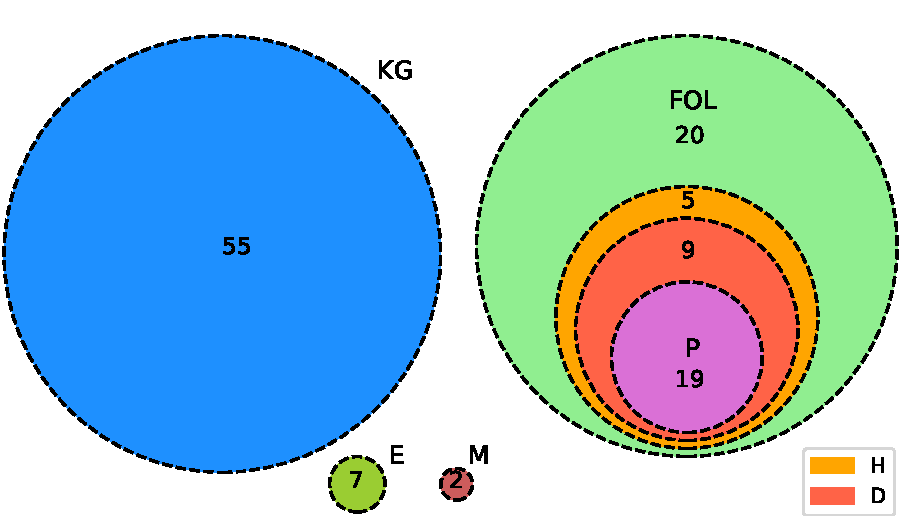
\includegraphics[width=.6\linewidth]{figures/ski-logic}
    \caption[Venn diagram categorising SKI methods w.r.t. the input knowledge type]{
        Venn diagram categorising SKI methods w.r.t.\ the \emph{input knowledge} type: knowledge graphs (KG), propositional logic (P), first-order logic (FOL), expert knowledge (E), Datalog (D), Horn logic (H), or modal logic (M).
        %
        The image is taken from~\cite{DBLP:journals/csur/CiattoSAMO24} and it refers to 117 surveyed \gls{SKI} methods.
    }
    \label{fig:pie-ski-logic}
\end{figure}
%
\note{ERROR: there is an inconsistency between this image and \Cref{fig:venn-diagram-logics}. P here is subset of D, there it is not.}
%
A key distinction in \gls{SKI} methods lies in whether the chosen formalism is \emph{machine interpretable}, \emph{human interpretable}, or both.
%
\Gls{SKI} methods can be categorized into two primary groups based on the formalism used to represent input knowledge~\cite{DBLP:journals/csur/CiattoSAMO24}:
%
\begin{itemize}
    \item \textbf{Logic formulas or \glspl{KB}:} These adhere to \gls{FOL} or its subsets, making them interpretable by both humans and machines.
    %
    The sub-categories, ordered by decreasing expressiveness, include:
    %
    \begin{itemize}
        %
        \item \emph{\gls{FOL} formulas:} These encompass recursive terms, variables, predicates of any arity, and various logic connectives, potentially expressing definitions.
        %
        \item \emph{Horn logic:} Often referred to as Prolog-like logic, this formalism consists of head–body rules involving predicates and terms of any kind.
        %
        \item \emph{Datalog:} A restricted subset of Horn logic that excludes recursive terms, allowing only constants or variables as terms.
        %
        \item \emph{Modal logics:} These extend the above logics with modal operators (e.g., \(\square\) and \(\lozenge\)), which express modalities such as necessity or possibility.
        %
        \item \emph{Knowledge graphs:} A practical application of description logics designed to represent entity–relation graphs.
        %
        \item \emph{Propositional logic:} This involves Boolean variables and logical connectives, offering a simpler yet effective formalism.
    \end{itemize}
    %
    \item \textbf{Expert knowledge:} This category includes human-interpretable knowledge that is not inherently machine-readable.
    %
    Examples include physics equations, syntactical rules, or domain-specific expertise.
    %
    Since expert knowledge is not directly machine interpretable, it often requires transformation into tensorial form through data generation, a process that typically involves human engineers and can be labor-intensive.
\end{itemize}
%
\Cref{fig:pie-ski-logic} illustrates the distribution of surveyed \gls{SKI} methods based on their formalism of choice.
%
\Glspl{KG} emerge as the most prevalent category, representing nearly half of the surveyed methods.
%
In contrast, modal logics constitute the smallest group.
%
Methods based on \gls{FOL} or its subsets (excluding \glspl{KG}) form another significant cluster, with propositional logic being particularly prominent due to its relative simplicity and widespread use.
%
The specific logic formalism employed in the surveyed papers is reported where available.
%
However, this information is rarely explicitly stated by the authors.
%
Instead, the logic is often inferred from the constraints and descriptions provided in the respective works.

Practical examples of symbolic knowledge that can be injected into sub-symbolic predictors are the public health guidelines on type-2 diabetes of the National Institute of Diabetes and Digestive and Kidney Diseases\footnote{\url{https://www.niddk.nih.gov/health-information/diabetes/}}.
%
These guidelines have been encoded into logic formulas~\cite{DBLP:conf/pkdd/KunapuliBSMS10} and used in works related to \gls{SKI}~\cite{Magnini-telmed2025}.
%
The first guideline state that if a patient has a glucose value greater or equal to 125 mg/dL and a \gls{BMI} greater or equal to 30, then the patient is considered diabetic.
%
The second one says that if a patient has a glucose value lower or equal to 100 mg/dL and a \gls{BMI} lower or equal to 25, then the patient is considered non-diabetic.
%
In \gls{FOL}, the first statement can be encoded as:
%
\begin{equation}\label{eq:rule-diabetic}
  \forall x . ( \text{glucose}(x) \geq 125 \land \text{bmi}(x) \geq 30 \rightarrow \text{Diabetic}(x))
\end{equation}
%
whereas the second statement can be encoded as:
%
\begin{equation}\label{eq:rule-not-diabetic}
  \forall x . ( \text{glucose}(x) \leq 100 \land \text{bmi}(x) \leq 25 \rightarrow \neg \text{Diabetic}(x))
\end{equation}


\subsection{Where to inject}\label{subsec:where-to-inject}
%
\begin{figure}
    \centering
    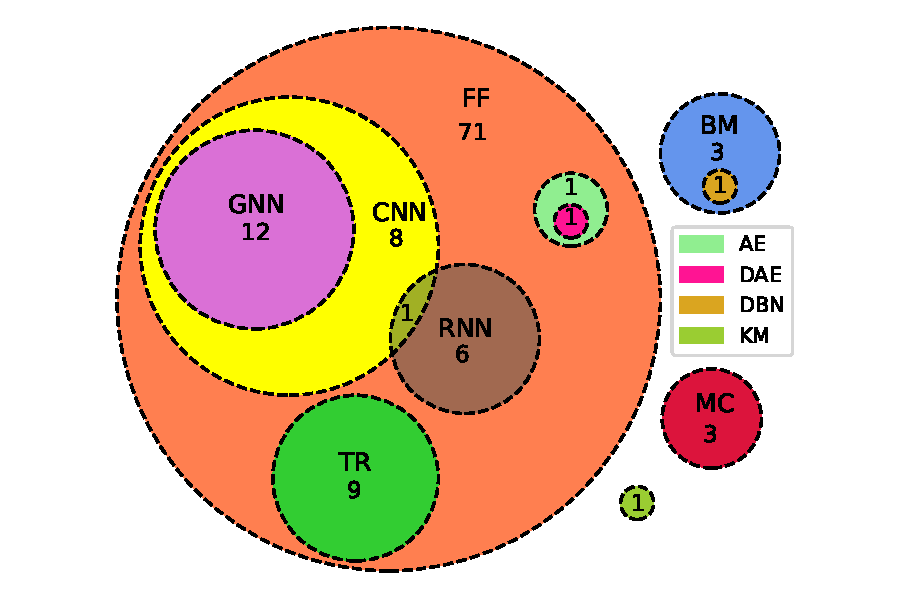
\includegraphics[width=.6\linewidth]{figures/ski-predictors}
    \caption[Venn diagram categorising SKI methods w.r.t. the type of sub-symbolic predictor]{
        Venn diagram categorising \gls{SKI} methods w.r.t.\ the type of sub-symbolic predictor: feed-forward (FF), convolutional (CNN), graph (GNN) or recurrent (RNN) neural networks, Boltzmann machines (BM), Markov chains (MC), transformers (TR), auto-encoders (AE), deep belief networks (DBN), denoising auto-encoders (DAE), kernel machines (KM).
        %
        The image is taken from~\cite{DBLP:journals/csur/CiattoSAMO24} and it refers to 117 surveyed \gls{SKI} methods.
    }
    \label{fig:pie-ski-predictors}
\end{figure}
%
\Gls{SKI} methods can target many different types of sub-symbolic predictors.
%
The vast majority of them are \glspl{NN}.
%
Among \glspl{NN}, there are different kinds of architectures that one can use to inject symbolic knowledge including.
%
In addition to \glspl{NN}, \gls{SKI} methods can also target other types of sub-symbolic predictors.
%
The predictors targeted by the surveyed \gls{SKI} methods are:
%
\begin{itemize}
    \item \textbf{feed-forward NNs} multi-layered \glspl{NN} in which neurons from layer i are only connected with layer i + 1, and multiple ($\ge$ 2) layers may exist;
    %
    \item \textbf{convolutional NNs} (CNNs) particular case of FF, \glspl{NN} that use convolutional layers to extract features from the input data, typically used in computer vision tasks;
    %
    \item \textbf{graph NNs} (GNNs) particular case of \glspl{CNN}, \glspl{NN} that operate on graph-structured data, allowing for the injection of symbolic knowledge in the form of graph structures;
    %
    \item \textbf{recurrent NNs} (RNNs) \glspl{NN} that use recurrent connections to process sequential data, such as time series or natural language;
    %
    \item \textbf{transformers} (TR) a type of \glspl{NN} architecture that uses self-attention mechanisms to process sequences, widely used in natural language processing tasks;
    %
    \item \textbf{auto-encoders} (AE) a type of \glspl{NN} that learns to encode input data into a lower-dimensional representation and then decode it back to the original input, often used for dimensionality reduction or feature extraction;
    %
    \item \textbf{denoising auto-encoders} (DAE) a type of auto-encoder that learns to reconstruct the original input from a corrupted version, often used for noise reduction or data augmentation;
    %
    \item \textbf{Boltzmann machines} (BM) a type of stochastic \glspl{NN} that can learn complex distributions over their inputs, often used for generative tasks;
    %
    \item \textbf{Markov chains} (MC) probabilistic models that represent systems that transition between states based on certain probabilities, often used for sequence prediction;
    %
    \item \textbf{deep belief networks} (DBN) a type of generative model that consists of multiple layers of stochastic, latent variables, often used for unsupervised learning tasks;
    %
    \item \textbf{kernel machines} (KM) a type of sub-symbolic predictor that uses kernel functions to map input data into a higher-dimensional space, allowing for non-linear decision boundaries.
\end{itemize}
%
\Cref{fig:pie-ski-predictors} illustrates the distribution of surveyed \gls{SKI} methods based on the type of sub-symbolic predictor they target.

One reason why the vast majority of methods rely on \glspl{NN} is straightforward: methods tailored to \glspl{GNN} (resp., \glspl{CNN}) assume the networks to accept specific kinds of data as input, e.g., graphs (resp., images), while ordinary feed-forward \glspl{NN} accept raw vectors of real numbers.
%
Another reason is that \glspl{NN} are the most popular sub-symbolic predictors in the \gls{ML} community, and they are often used as a default choice for many tasks.
%
Finally, \glspl{NN} are highly flexible and easy to manipulate, making them ideal for \gls{SKI} methods.


\subsection{How to inject}\label{subsec:how-to-inject}
%
\begin{SCfigure}
    \centering
    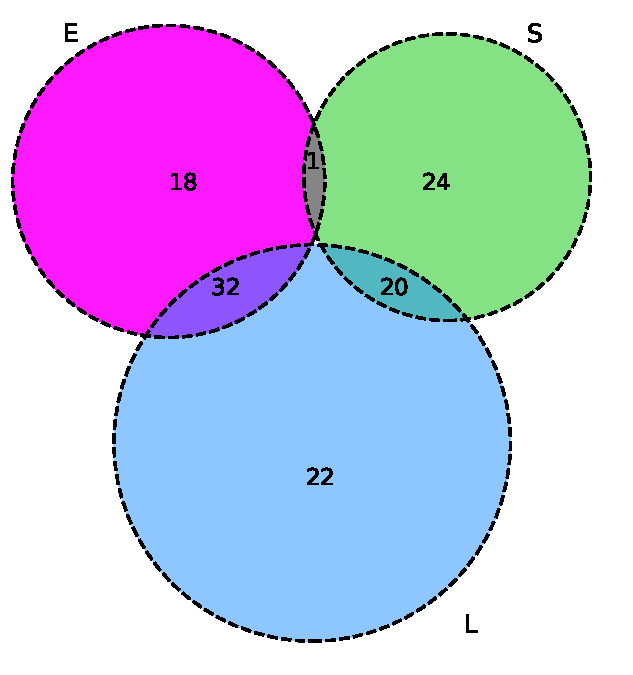
\includegraphics[width=.4\linewidth]{figures/ski-integration}
    \caption[Venn diagram categorising SKI methods]{
        Venn diagram categorising SKI methods w.r.t.\ the \emph{injection} strategy type: structuring (S), embedding (E), or guided learning (L).
        %
        The image is taken from~\cite{DBLP:journals/csur/CiattoSAMO24} and it refers to 117 surveyed \gls{SKI} methods.
    }
    \label{fig:pie-ski-injection}
\end{SCfigure}
%
How can symbolic knowledge, such as the ones in \Cref{eq:rule-diabetic,eq:rule-not-diabetic}, be injected into sub-symbolic predictors?
%
To answer this question, scientists have designed several strategies, which can be broadly grouped into three main categories~\cite{DBLP:journals/csur/CiattoSAMO24}: structuring, guided learning, and embedding.
%
It may occur that a method uses more than one strategy at a time.
%
\Cref{fig:pie-ski-injection} illustrates the distribution of surveyed \gls{SKI} methods based on their strategy of choice.
%
The survey revealed that all three strategies are widely used, with learning being the most frequent but not dominant.

The main entities involved in the \gls{SKI} process -- and that are common to virtually all \gls{SKI} methods -- are:
%
\begin{itemize}
    %
    \item \textbf{symbolic knowledge:} in the vast majority of cases, this is a set of logic formulas or a \gls{KB} that encodes the symbolic knowledge to be injected;
    %
    \item \textbf{parsed knowledge:} a syntactic structure that represents the \emph{parsed} symbolic knowledge, often in the form of a \gls{AST} or graph;
    %
    \item \textbf{sub-symbolic component:} a sub-symbolic instance built upon the parsed symbolic knowledge;
    %
    \item \textbf{uneducated sub-symbolic predictor:} a sub-symbolic predictor that has not been enriched with the symbolic knowledge;
    %
    \item \textbf{educated sub-symbolic predictor:} the final sub-symbolic predictor that has been enriched with the symbolic knowledge.
    %
\end{itemize}
%


\paragraph{Structuring}\label{par:structuring}
%
\begin{figure}
    \centering
    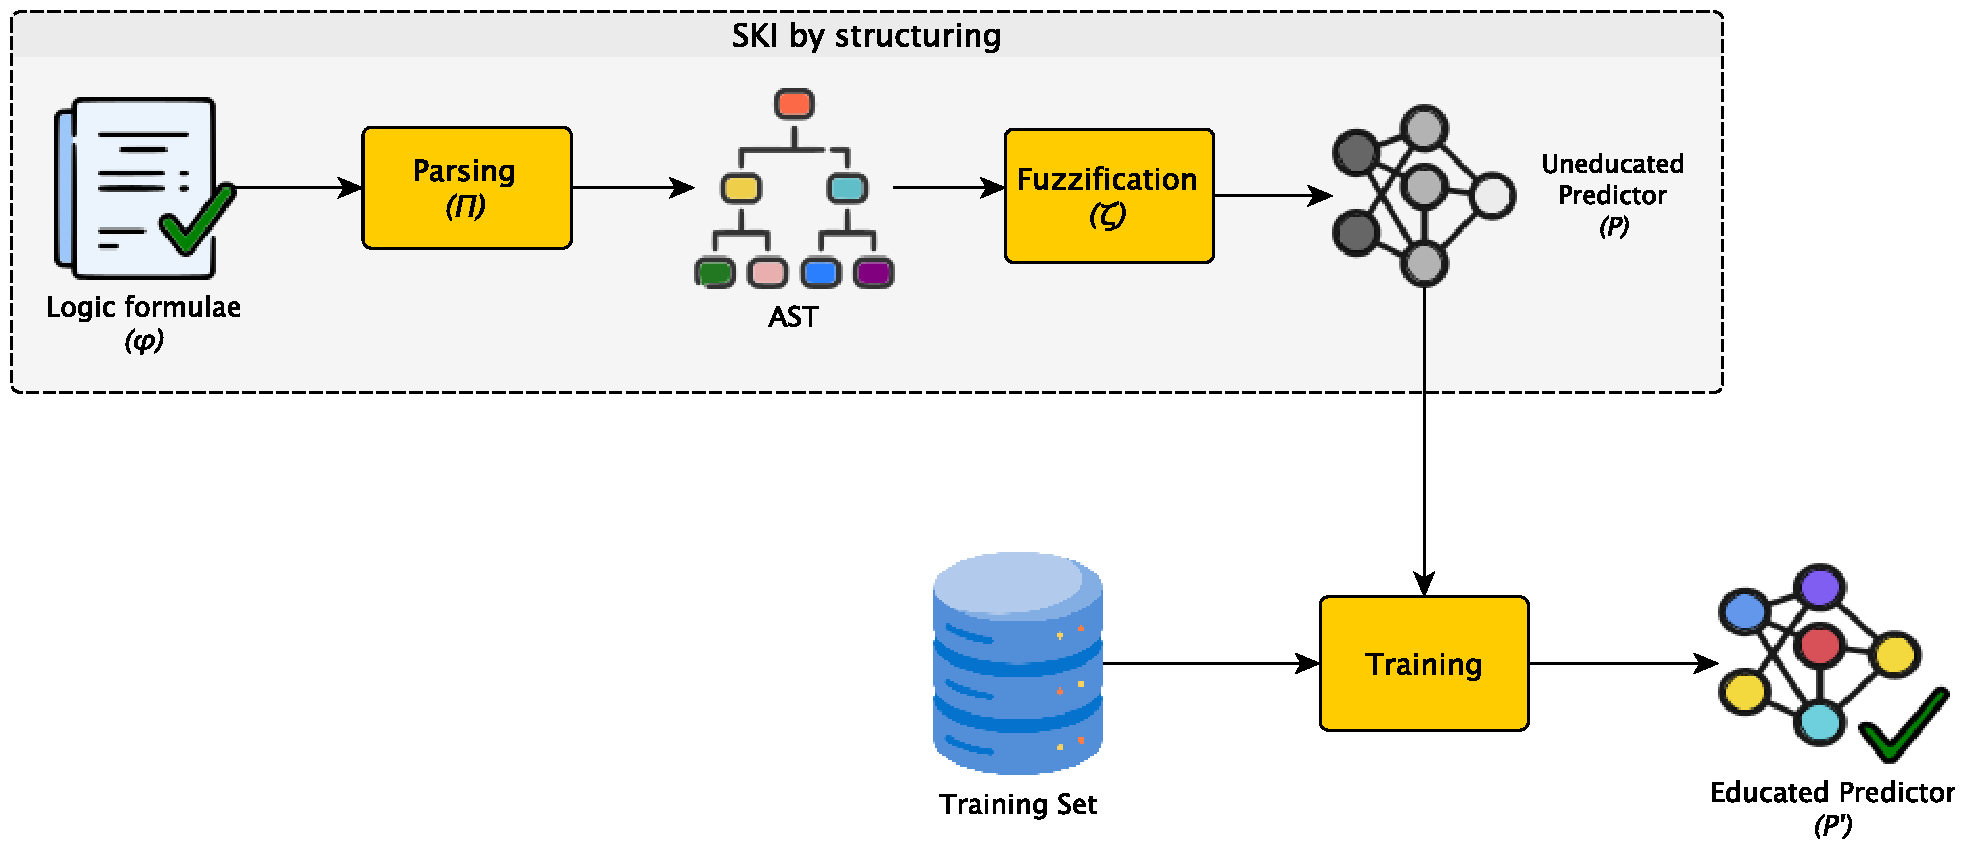
\includegraphics[width=.9\linewidth]{figures/workflow-structuring}
    \caption[SKI workflow of structuring strategy]{
        Workflow of the structuring strategy.
        %
        The symbolic knowledge is parsed and used to create a sub-symbolic predictor -- or part of it -- that mimics the symbolic knowledge.
        %
        The resulting predictor is then trained on data, if needed.
    }
    \label{fig:workflow-structuring}
\end{figure}
%
By predictor structuring, or simply structuring, we identify all those methods that use a part (or the whole) of a sub-symbolic predictor to \emph{mirror} the symbolic knowledge via its own internal structure.
%
A predictor is either created or extended to mimic the behavior of the symbolic knowledge.
%
For instance, when the predictors are \glspl{NN}, their internal structure is crafted to represent logic predicates via neurons, and logic connectives via synapses.
%
\Cref{fig:workflow-structuring} illustrates the workflow of the structuring strategy.
%
Usually, in the structuring strategy, the symbolic knowledge is in the form of logic formulas ($\phi$) (e.g., subsets of \gls{FOL}).
%
The formulas are then parsed into a syntactic structure (e.g., \gls{AST}).
%
At this point, a \emph{fuzzification} ($\zeta$) step is performed to convert the \emph{boolean} (also the term \emph{crisp} is used in the literature) -- because a logic predicate is either \emph{true} or \emph{false} -- symbolic knowledge into a \emph{fuzzy} interpretation of it, which is more suitable for sub-symbolic predictors.
%
This fuzzy interpretation is often \emph{continuous} and bounded to a predefined range, such as \([0, 1]\).
%
The property of continuity is a key requirement for training sub-symbolic structures via gradient descent (e.g., \glspl{NN} or part of them).
%
In practice, $\zeta$ is implemented as a mapping function that transforms logic operators into continuous functions (see \Cref{sec:from-symbolic-to-sub-symbolic}).
%
The result of the fuzzification process is an \emph{uneducated} predictor ($P$) that is then trained on the training set.
%
After the training, the predictor is now \emph{educated} ($P'$) and can be used to make predictions on the test set or in production.
%

\paragraph{Guided learning}\label{par:guided-learning}
%
\begin{figure}
    \centering
    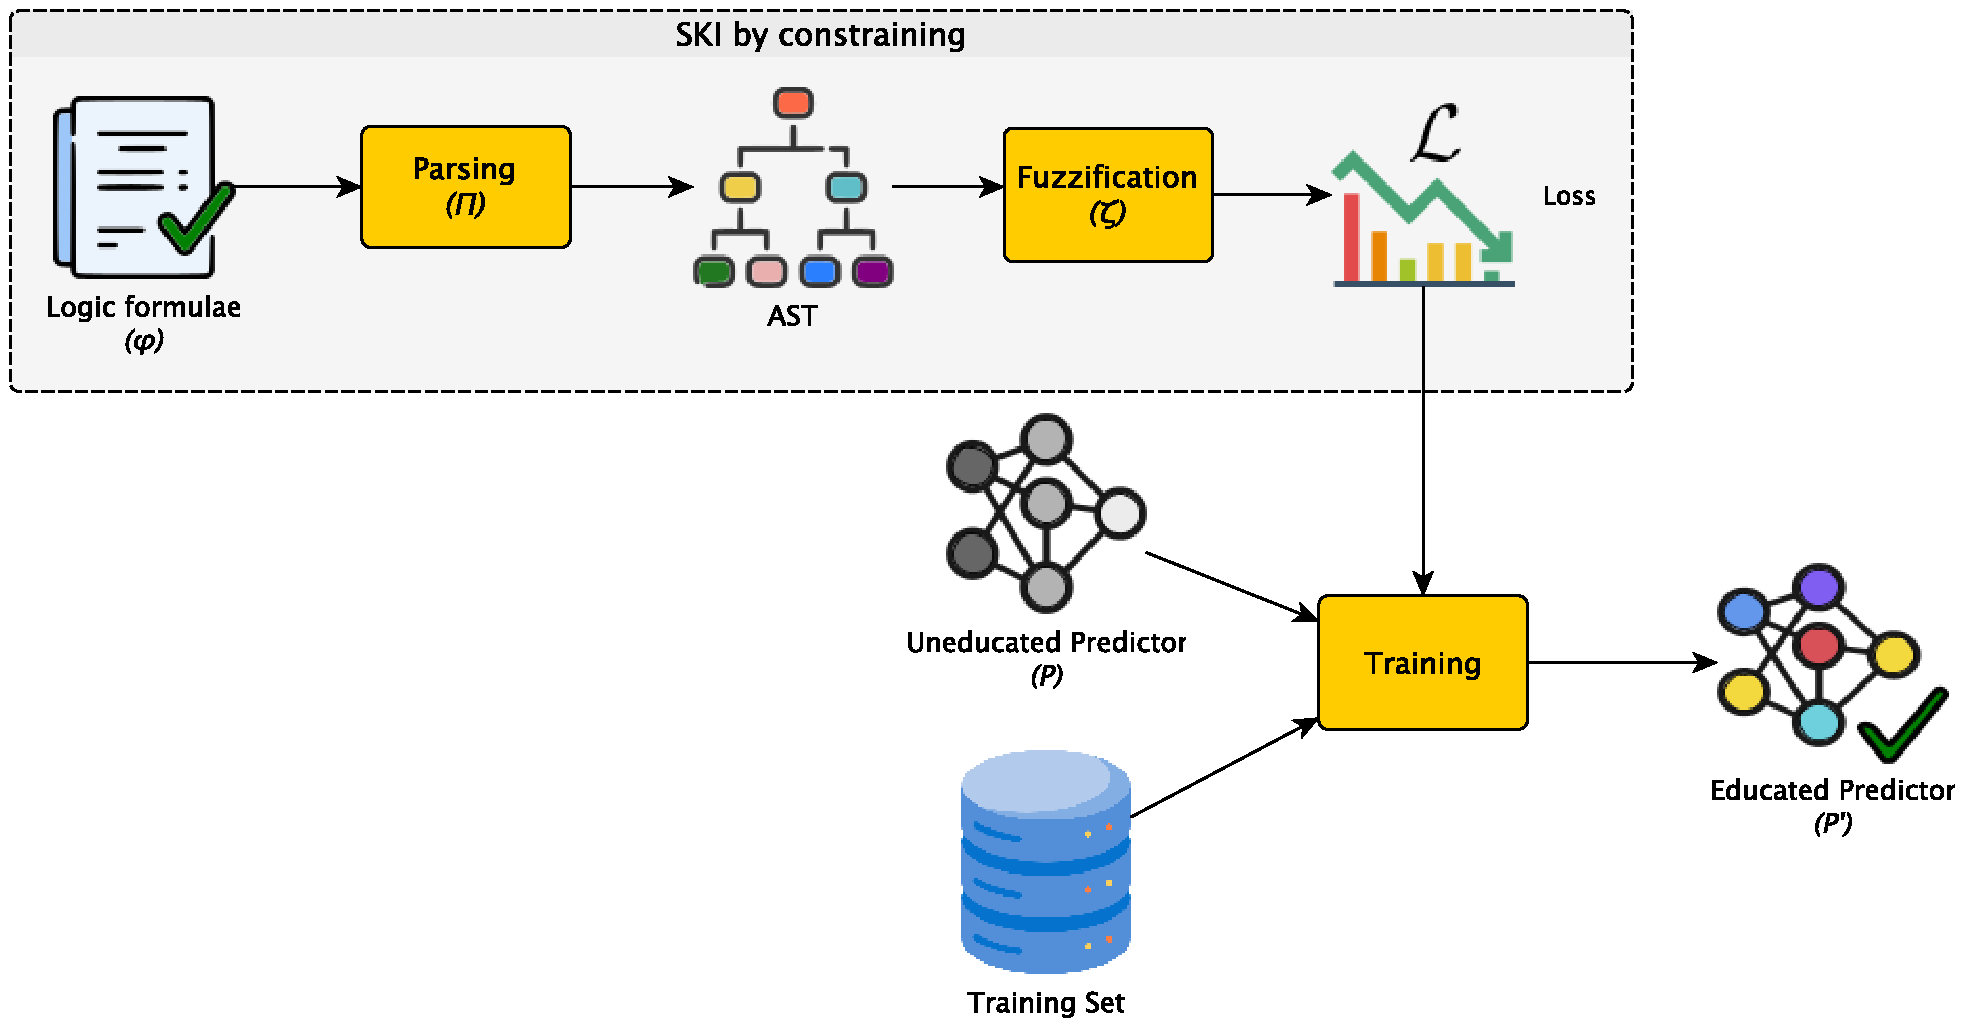
\includegraphics[width=.9\linewidth]{figures/workflow-constraining}
    \caption[SKI workflow of guided learning strategy]{
        \gls{SKI} workflow of the guided learning strategy.
        %
        The symbolic knowledge is used to guide the training of a sub-symbolic predictor, which is then trained on data.
    }
    \label{fig:workflow-learning}
\end{figure}
%
By guided learning, we refer to all those methods that affect the sub-symbolic predictor's training process by using the symbolic knowledge as a \emph{constraint}/\emph{guidance}.
%
Usually, \gls{SKI} algorithms based on this strategy target sub-symbolic predictors that can be trained with gradient descent, such as \glspl{NN}.
%
\Cref{fig:workflow-learning} illustrates the workflow of the guided learning strategy.
%
Like in the case of structuring, the symbolic knowledge is parsed and fuzzified.
%
Differently from structuring, the result of the fuzzification process is not a subcomponent of the predictor's architecture (e.g., neurons, connections), but rather a set of continuous numeric functions.
%
Conceptually, these functions represent the degree of violation of the symbolic knowledge by the predictor's predictions.
%
The higher the degree of violation, the higher the value of the function.
%
The symbolic-derived functions are then included in the loss function of the predictor, which is then trained on the training set.
%
The combination between the ``classical'' loss function (e.g., cross-entropy, mean squared error, etc.) and the symbolic-derived functions can be done in many ways, but it is usually done via a weighted sum.


\paragraph{Embedding}\label{par:ski-embedding}
%
\begin{figure}
    \centering
    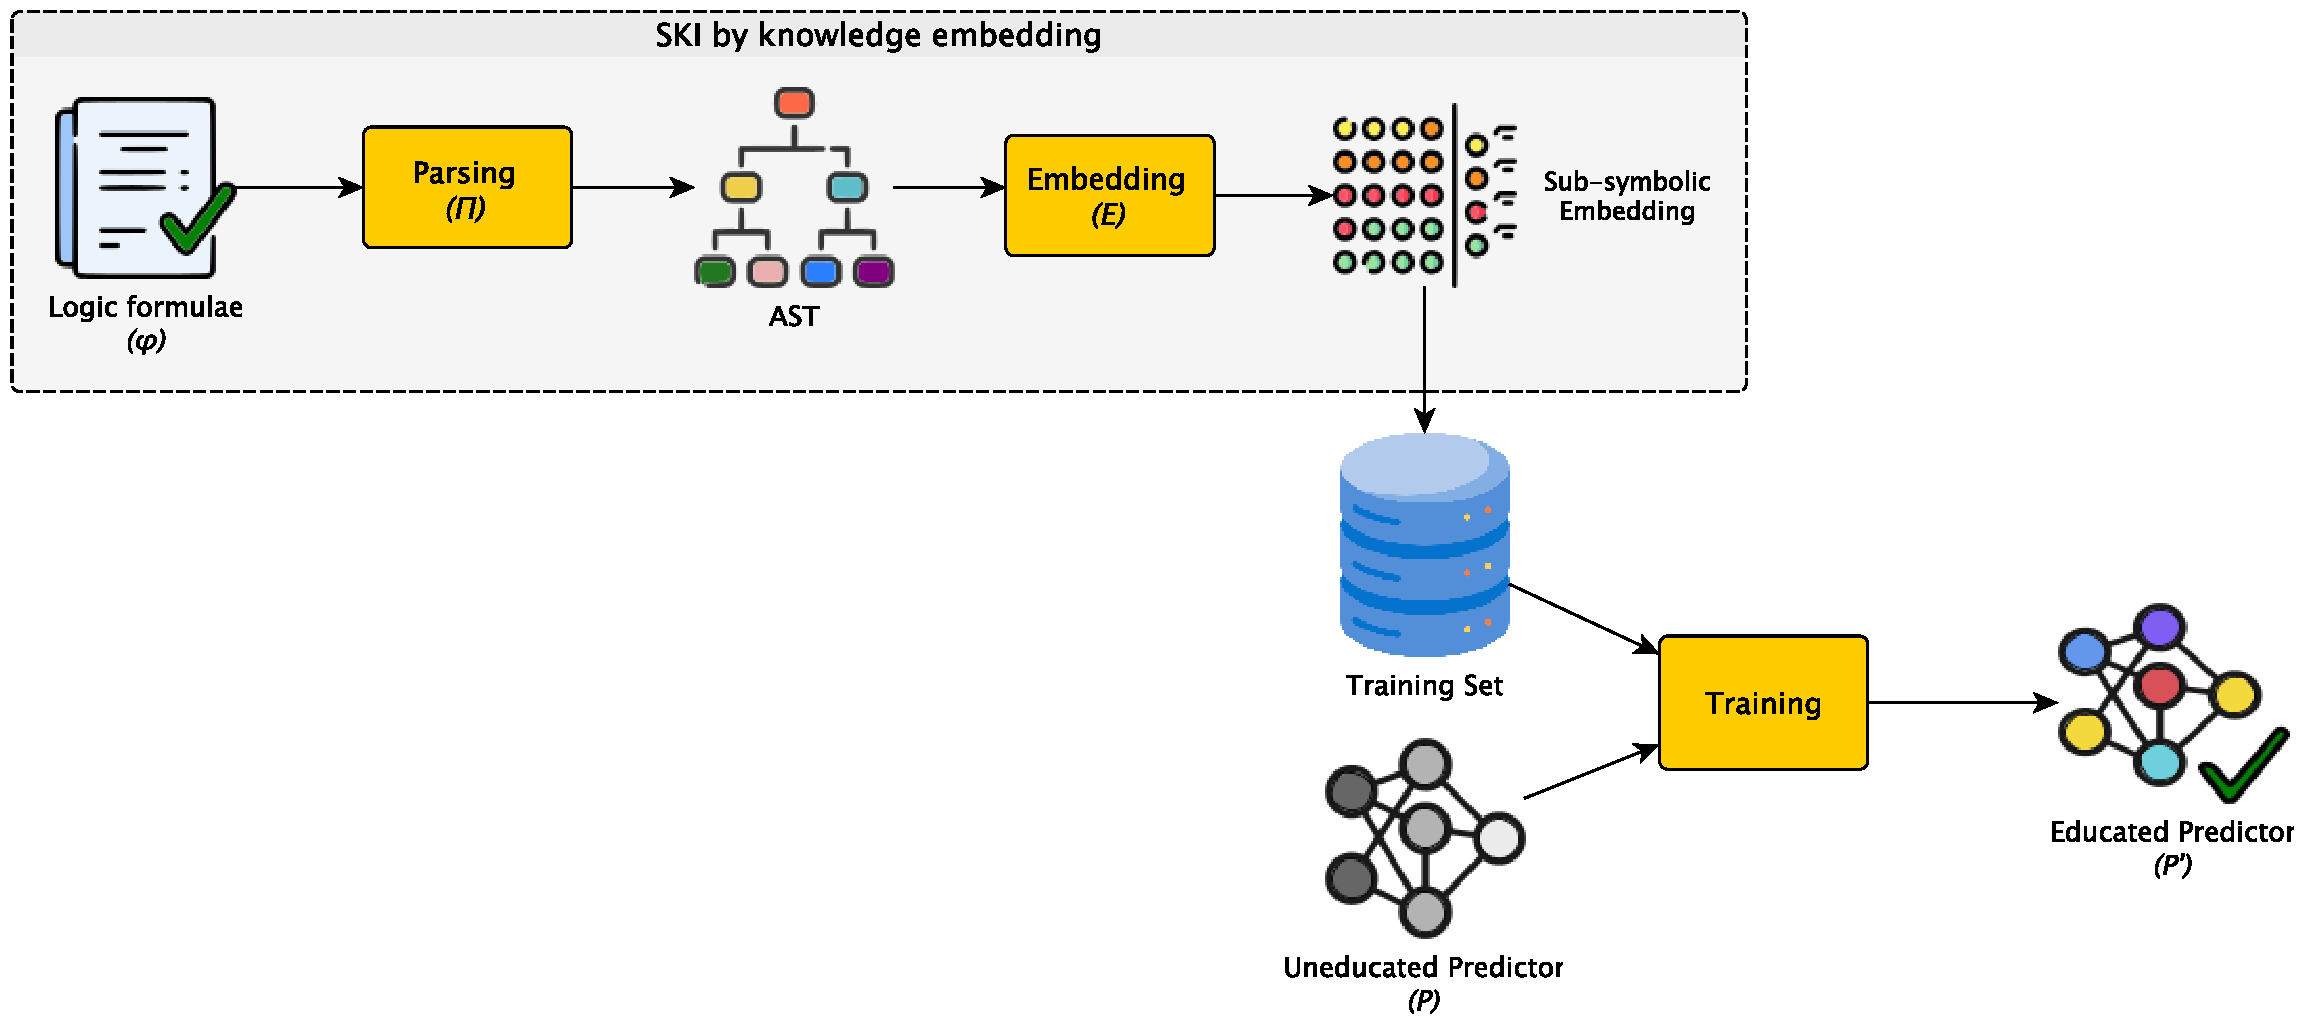
\includegraphics[width=.9\linewidth]{figures/workflow-embedding}
    \caption[SKI workflow of embedding strategy]{
        \gls{SKI} workflow of the embedding strategy.
        %
        The symbolic knowledge is parsed and embedded into a sub-symbolic predictor, which is then trained on data.
    }
    \label{fig:workflow-embedding}
\end{figure}
%
In the embedding strategy, the symbolic knowledge is converted -- i.e., \emph{embedded}-- into numeric-array representations.
%
\Cref{fig:workflow-embedding} illustrates the workflow of the embedding strategy.
%
The output of the fuzzification process is a set of numeric arrays (e.g., vectors, matrices, and tensors) that represent the symbolic knowledge.
%
These arrays are then provided as input to the sub-symbolic predictor.
%
This is the common strategy exploited by the \gls{KG}~\cite{DBLP:conf/ijcai/LambGGPAV20} embedding community as well as by \glspl{GNN}~\cite{DBLP:journals/tkde/WangMWG17}.


\subsection[Limitations and challenges of SKI]{Limitations and challenges of \Gls{SKI}}\label{subsec:limitations-and-challenges-of-ski}


\section[Symbolic knowledge extraction]{\Glsentrylong{SKE}}\label{sec:ske}
%
\gls{SKE} is the process of extracting symbolic knowledge from sub-symbolic predictors.
%
Here, we provide the broad definition of \gls{SKE} that we adopt in this thesis:
%
\begin{definition}[\gls{SKE}]
    \label{def:ske}
    any \textbf{algorithmic} procedure accepting \textbf{trained} sub-symbolic predictors as input and producing \textbf{symbolic} knowledge as output so that the extracted knowledge reflects the behavior of the predictor with high \textbf{fidelity}~\cite{DBLP:journals/csur/CiattoSAMO24}.
\end{definition}
%
Once again, the definition is broad because the amount of contributions in the literature is vast and varied, they often use different terminologies and come from different communities.
%
\Gls{SKE} is conceptualized as a class of algorithms, which are finite-step procedures defined by their inputs and outputs.

The input to \gls{SKE} procedures must be trained \glspl{ML} predictors.
%
There are no restrictions on the type of predictor, meaning that \gls{SKE} methods can, in principle, be applied to any predictor family.
%
However, this requirement implies that the predictor must have already undergone training and achieved satisfactory performance for its intended task.
%
Thus, within an \gls{ML} workflow, \gls{SKE} is performed after the training and validation phases are complete.

The output of \gls{SKE} procedures is symbolic knowledge, which is broadly defined as human-intelligible information.
%
This can include logic formulas, decision trees, or even plain human-readable text.
%
For an algorithm to qualify as a valid \gls{SKE} procedure, the extracted knowledge must closely reflect the behavior of the original predictor within the domain it was trained for.
%
This fidelity is typically measured using a fidelity score, which evaluates how well the extracted knowledge replicates the predictor's behavior for the given task and domain.

The extracted knowledge should ideally function as a predictor itself, allowing it to be queried in the same way as the original predictor.
%
For example, if the original predictor is an image classifier, the extracted knowledge should enable an intelligent agent to classify similar images and produce equivalent results.
%
This agent could be either computational (e.g., a software program) or human, depending on whether the extracted knowledge is machine or human interpretable.
%
The use of logic-based knowledge as the target of \gls{SKE} is particularly advantageous, as it supports both machine and human interpretability.


\subsection{Motivations and goals}\label{subsec:ske-motivations-and-goals}
%
\Gls{SKE} serves multiple purposes, including:
%
\begin{inlinelist}
    %
    \item \label{itm:inspection} the inspection of the internal operations of opaque predictors, which are otherwise treated as black boxes,
    %
    \item \label{itm:automation} the automation and acceleration of the process of acquiring symbolic knowledge, eliminating the need for manually crafting \glspl{KB},
    %
    \item \label{itm:xai} providing valuable capabilities within the scope of \gls{XAI} to analyze black-box predictors.
\end{inlinelist}

\Cref{itm:inspection} is particularly important for understanding the behavior of opaque predictors.
%
By inspecting their internal operations, \gls{SKE} allows researchers and practitioners to identify patterns in mispredicted inputs or even detect correctly predicted patterns that rely on unethical or biased decision processes.
%
This capability is crucial for ensuring the ethical and transparent use of \gls{ML} systems, especially in sensitive domains such as healthcare or finance.

\Cref{itm:automation} highlights another key advantage of \gls{SKE}: the ability to automate the extraction of symbolic knowledge.
%
This eliminates the labor-intensive process of manually crafting \glspl{KB}, which often requires significant domain expertise and time.
%
By automating this process, \gls{SKE} not only accelerates knowledge acquisition but also enables the reuse of extracted knowledge across different tasks or systems, provided the knowledge is represented in a compatible format.

Finally, \Cref{itm:xai} emphasizes the role of \gls{SKE} in \gls{XAI}.
%
The extracted knowledge can be used to construct explanations for the behavior of black-box predictors, making their decision-making processes more interpretable.
%
In some cases, this knowledge may even serve as an interpretable surrogate model, replacing the original predictor if it achieves a high fidelity score~\cite{DBLP:conf/atal/CiattoCSO20}.
%
Additionally, \gls{SKE} enables the comparison of multiple black-box predictors performing the same task, highlighting their differences and commonalities.
%
It also facilitates the merging of knowledge extracted from various predictors, even if they belong to different families, as long as the same representation format is used~\cite{DBLP:conf/aiia/CiattoCOC19}.


\subsection{What to extract}\label{subsec:what-to-extract}
%
\begin{figure}
    \centering
    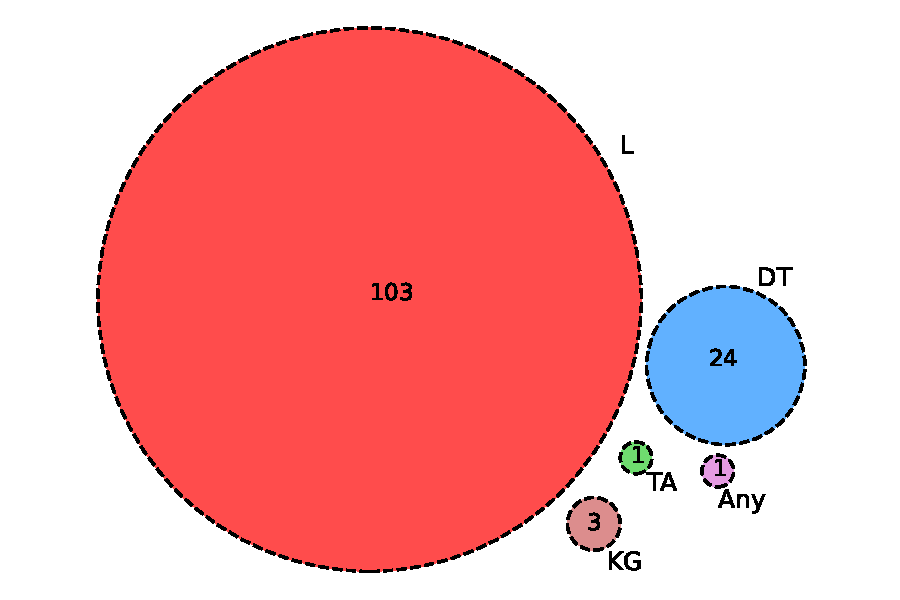
\includegraphics[width=.6\linewidth]{figures/ske-rule-shape}
    \caption[Venn diagram categorising SKE methods]{
        %
        Venn diagram categorising \gls{SKE} methods w.r.t.\ the \emph{shape} of the extracted symbolic knowledge: rule lists (L), decision trees (DT), decision tables (TA), or knowledge graphs (KG).
        %
        The image is taken from~\cite{DBLP:journals/csur/CiattoSAMO24} and it refers to 132 surveyed \gls{SKE} methods.
    }
    \label{fig:pie-ski-shape}
\end{figure}
%
\begin{figure}
    \centering
    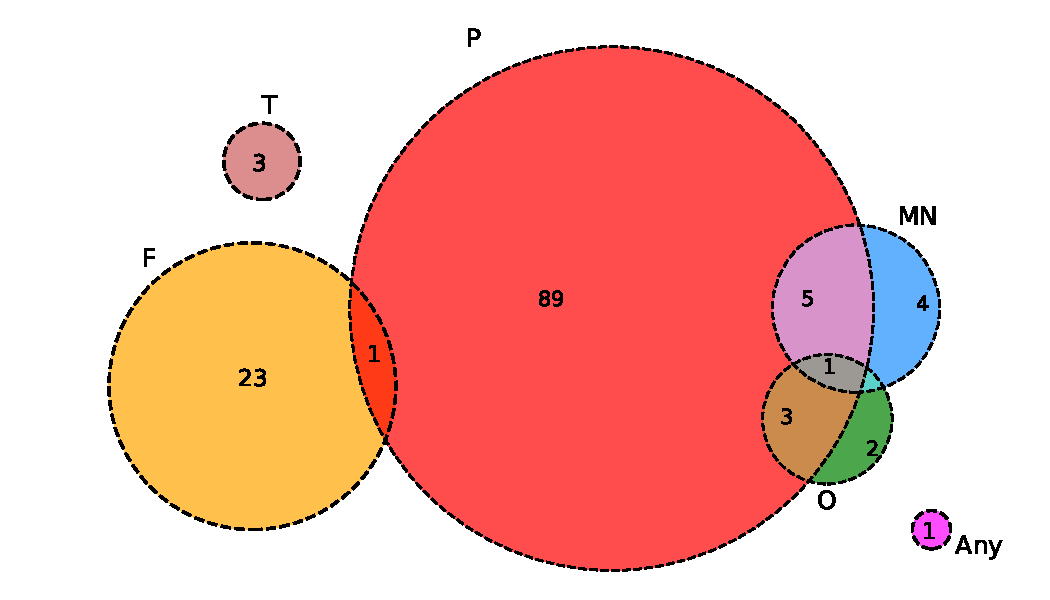
\includegraphics[width=.6\linewidth]{figures/ske-rule-format}
    \caption[Pie chart categorising SKE methods]{
        %
        Pie chart categorising \gls{SKE} methods w.r.t.\ the semantic \emph{expressiveness} of the extracted symbolic knowledge: propositional rules (P), fuzzy rules (F), oblique rules (O), m-of-n rules (MN), or triplets (T).
        %
        The image is taken from~\cite{DBLP:journals/csur/CiattoSAMO24} and it refers to 132 surveyed \gls{SKE} methods.
    }
    \label{fig:pie-ski-expressiveness}
\end{figure}

What kind of symbolic knowledge can be extracted?
%
Symbolic knowledge extracted from \glspl{ML} predictor should ideally mimic the behavior of the predictor itself.
%
For supervised \gls{ML}, this means that the extracted knowledge should represent a function mapping input features to output features, such as classes in classification tasks.
%
These functions can be expressed in symbolic formats, which vary in both syntax and semantics.

\paragraph{Shape of the extracted knowledge}
%
From a syntactic perspective, the shape of the extracted symbolic knowledge is crucial for its interpretability.
%
The most common formats include decision rules and decision trees, as they are widely recognized for their human-comprehensibility.
%
Other formats, such as decision tables and knowledge graphs, are also used, though less frequently.
%
Regardless of the format, the extracted knowledge typically uses symbols to represent the same input and output features as the original \gls{ML} predictor.

We identify four primary syntactic shapes for extracted symbolic knowledge:
%
\begin{itemize}
    \item \textbf{Lists of rules:} Sequences of logic rules presented in a predefined order.
    %
    \item \textbf{Decision trees:} Hierarchical structures where each node represents a decision rule (see \Cref{subsec:decision-trees}).
    %
    \item \textbf{Decision tables:} Tabular representations specifying conclusions for different sets of conditions.
    %
    These can be exhaustive, listing all possible combinations, or incomplete, covering only a subset of cases.
    %
    Each row (or column) corresponds to a rule, with cells indicating variable values.
    %
    An example is provided in the supplementary material.
    %
    \item \textbf{Knowledge graphs:} Graph-based representations of entities and their relationships (see \Cref{subsec:ontologies-and-kg}).
\end{itemize}

\Cref{fig:pie-ski-shape} illustrates the distribution of these shapes across surveyed \gls{SKE} methods.
%
Rule lists are the most prevalent, likely due to their simplicity and algorithmic tractability.

\paragraph{Expressiveness of the extracted knowledge}
%
From a semantic perspective, the expressiveness of the extracted symbolic knowledge depends on the logical constructs it employs.
%
Statements may include predicates, relations, logic connectives, and arithmetic comparators, which determine what can be expressed.
%
We categorize the semantic formats of extracted symbolic knowledge as follows:
%
\begin{itemize}
    \item \textbf{Propositional rules:} Statements involving Boolean input/output features connected by logic operators such as negation, conjunction, and disjunction.
    %
    Arithmetic comparisons between continuous features and constants are also included in this category.
    %
    \item \textbf{Fuzzy rules:} Extensions of propositional rules where truth values range continuously between 0 and 1.
    %
    \item \textbf{Oblique rules:} Rules with conditions expressed as inequalities involving linear combinations of input variables, allowing comparisons between features.
    %
    \item \textbf{m-of-n rules:} Rules that are true if at least \(m\) out of \(n\) conditions are satisfied.
    %
    These are a concise way of representing disjunctions of conjunctions.
    %
    \item \textbf{Triplets:} Representations commonly used in knowledge graphs, consisting of subject-predicate-object triples (see \Cref{subsec:ontologies-and-kg}).
\end{itemize}

\Cref{fig:pie-ski-expressiveness} summarizes the occurrence of these semantic formats in surveyed \gls{SKE} methods.
%
Propositional rules dominate due to their simplicity and tractability.
%
They allow a divide-and-conquer approach, focusing on one input feature at a time, which simplifies the extraction process.


\subsection{Where to extract}\label{subsec:where-to-extract}
%
\begin{figure}
    \centering
    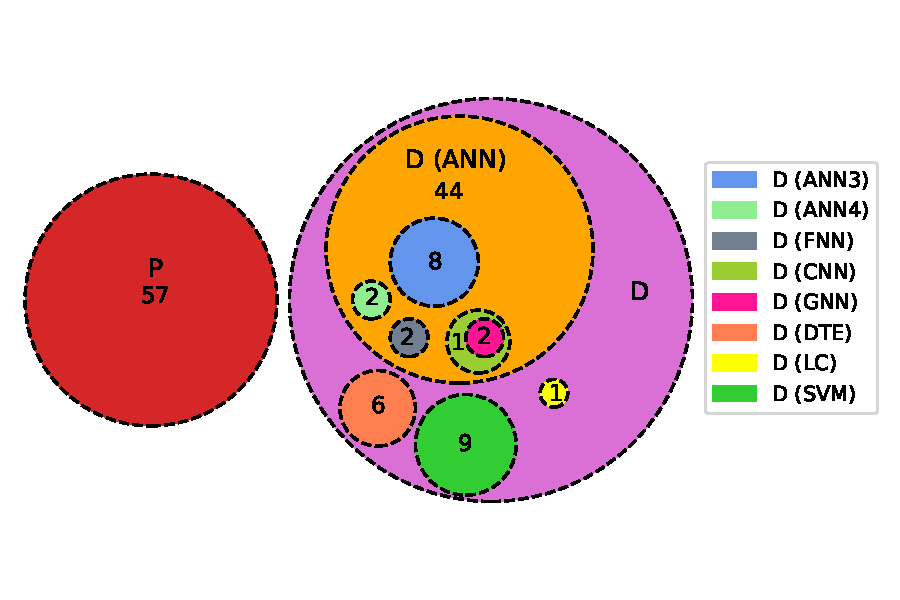
\includegraphics[width=.6\linewidth]{figures/ske-translucency}
    \caption[Venn diagram categorising SKE methods]{
        %
        Venn diagram categorising \gls{SKE} methods w.r.t.\ the \emph{translucency} of the algorithm: decompositional (D) or pedagogical (P).
        %
        For decompositional methods, we report the target predictor type: ANN\<n\> = artificial \gls{NN} (possibly having exactly \<n\> layers), CNN = convolutional \gls{NN}, GNN = graph \gls{NN}, FNN = fuzzy \gls{NN}, SVM = support vector machines, DTE = decision tree ensembles, LC = linear classifiers.
        %
        The image is taken from~\cite{DBLP:journals/csur/CiattoSAMO24} and it refers to 132 surveyed \gls{SKE} methods.
    }
    \label{fig:pie-ske-translucency}
\end{figure}
%
The sort of \gls{ML} predictors from which symbolic knowledge can be extracted is strongly related to the \emph{translucency} of the \gls{SKE} algorithms.
%
The translucency of a \gls{SKE} algorithm refers to its ability to access the internal structure of the predictor, such as its parameters, weights, and architecture.
%
So, in other words, the question of where to extract symbolic knowledge is related to the question of how \gls{SKE} algorithms work.
%
There are two ways for \gls{SKE} methods to deal with sub-symbolic predictors:
%
\begin{itemize}
    \item \textbf{Decompositional} $\rightarrow$ if the method needs to inspect -- even partially -- the internal structure of the predictor, such as its parameters, weights, and architecture;
    %
    \item \textbf{Pedagogical} $\rightarrow$ if the method does not need to inspect the internal structure of the predictor, but rather it can treat it as a black box and it relies on the input/output behavior of the predictor.
\end{itemize}

The different nature of decompositional \gls{SKE} methods is detailed in \Cref{fig:pie-ske-translucency}.
%
We observe that for what concern decompositional methods, the vast majority of them are designed to work with \gls{NN} of various types and different number of hidden layers.
%
Also \glspl{SVM} and \glspl{DTE} are targeted by some decompositional methods.
%
Around 43\% of the surveyed methods are pedagogical, meaning that these methods can work with virtually any type of sub-symbolic predictor, as long as it can be queried for input/output pairs.
%
Therefore, in general \gls{SKE} methods can be applied to any type of predictor, but for the decompositional ones, \glspl{NN} are definitely the most targeted type.


\subsection{How to extract}\label{subsec:how-to-extract}
%
The way \gls{SKE} methods extract symbolic knowledge highly depends on the translucency of the method itself.
%
Pedagogical methods treat the underlying predictor as an oracle to be queries for predictions the symbolic knowledge should mimic.
%
\note{TODO: add citations}
%
In most of these cases, the \gls{SKE} method exploits a \emph{surrogate} model, which is a simpler, more interpretable model that approximates the behavior of the original predictor.
%
This model can be used as the final output of the \gls{SKE} process if it is already in a symbolic or interpretable (e.g., a linear model) format, or it can be further processed to extract symbolic knowledge.
%
Decompositional methods, on the other hand, require access to the internal structure of the predictor and each method has its own way of extracting symbolic knowledge.
%
\note{TODO: does it make sense to talk about this here?}
%
Another important aspect of \gls{SKE} methods when it comes to how symbolic knowledge is extracted is the \emph{granularity} of the extraction.

\paragraph{Local explanations}\label{par:local-explanations}
%
\begin{figure}
    \centering
    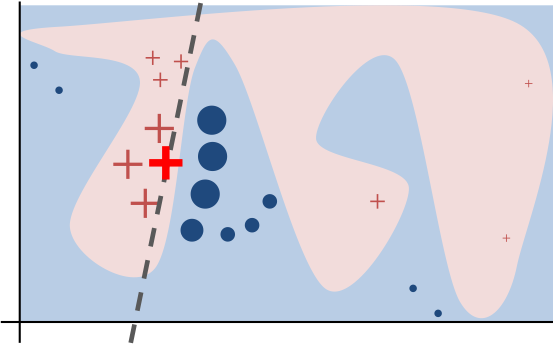
\includegraphics[width=.6\linewidth]{figures/local-explanation}
    \caption[Local explanations]{
        %
        Simple example to of how a local explanation can be provided for a specific input.
        %
        The sub-symbolic model's decision function $f$ is represented by the blue and pink background, which cannot be approximated well by a linear model.
        %
        The bold red cross is the instance being explained.
        %
        A \gls{SKE} method can sample inctances, get prediction using $f$, and weights them by the proximity to the instance being explained (the bigger the cross/circle, the closer to the instance).
        %
        The dashed line is the trained interpretable model that is locally faithful to the sub-symbolic model.
        %
        The image is taken from~\cite{DBLP:conf/kdd/Ribeiro0G16}.
    }
    \label{fig:local-explanations}
\end{figure}
%
When the interest in the extracted symbolic knowledge is focused on a specific input, i.e., we want to know why a predictor produced a particular outcome, the \gls{SKE} method is said to produce \emph{local explanations}.
%
A local explanation is symbolic knowledge that explains only the behavior of the predictor for a specific input.
%
The knowledge is not necessary encoded into logic rules, it can be provided for instance through \emph{feature importance} scores, which indicate the relevance of each input feature for the prediction~\cite{DBLP:conf/kdd/Ribeiro0G16}.
%
\Cref{fig:local-explanations} illustrates a simple example of how a local explanation can be provided for a specific input using a pedagogical \gls{SKE} method.


\paragraph{Global explanations}\label{par:global-explanations}
%
Conversely, when the interest is in understanding the overall behavior of the predictor, we say that the \gls{SKE} method produces \emph{global explanations}.
%
Global explanations aim to capture the general patterns and rules that govern the predictor's behavior across all inputs, rather than focusing on individual instances.
%
For example, this can be done by training a surrogate model -- if we want to use a pedagogical \gls{SKE} method -- using for instance the training set used to train the predictor.
%
However, instead of using the labels of the training set, the surrogate model is trained using the predictions of the original predictor.


\subsection[Limitations and challenges of SKE]{Limitations and challenges of \Gls{SKE}}\label{subsec:limitations-and-challenges-of-ske}